\chapter{Appendix}
\label{chapter7}
\section{Jacobi-Anger identity}
\label{sec:jacobi-anger}
Taking the generating function of the Bessel functions
\begin{equation}
\exp\left\{\frac{1}{2} z \left(t - t^{-1}\right)\right\} = \sum_{m=-\infty}^\infty t^m J_m(z)
\end{equation}
we can make the substitution $t = \exp \{i \omega t'\}$.
This gives the Jacobi-Anger expansions, which are useful for expanding sinusoidal phase modulation in terms of sidebands around the carrier:
\begin{align}
e^{i\Gamma\cos\Omega t} & = \sum_{n=-\infty}^{\infty} \left(i^n\right)  J_n(\Gamma) \exp\{i n \Omega t\} \\
e^{i\Gamma\sin\Omega t} & = \sum_{n=-\infty}^{\infty} J_n(\Gamma) \exp\{i n \Omega t\}
\end{align}


\section{The difference between PM and AM}
\label{sec:am-vs-pm}
%
Suppose we have a signal consisting of a carrier (at frequency $\omega$ and
with unit amplitude) and two sidebands, of amplitudes $a$ (lower) and $b$
(upper), separated from the carrier by a frequency $\Omega$:
%
\begin{equation}
E(t) = \left(1 + a \exp(-i \Omega t) + b \exp(i \Omega t)\right)
\exp(i \omega t)
\end{equation}
%
To find the power in this signal, we take the
modulus squared, $P = E^*E$ where * is the complex conjugate:
%
\begin{equation}
\begin{split}
P = & \left(1 + |a|^2 + |b|^2\right) \\
    & + \left(a^* + b\right) \exp(-i \Omega t) + \left(a + b^*\right) \exp(i \Omega t) \\
    & + \left(ab^*\right) \exp(-2 i \Omega t) + \left(a^*b\right) \exp(2 i \Omega t)
\end{split}
\end{equation}
%
The condition for the $1\Omega$ variation in the power to vanish is
$a=-b*$, i.e. the real parts of the amplitudes of the sidebands must
be opposite, and the imaginary parts must be equal. So we can extract
the amplitude and phase modulation indicies:
%
\begin{equation}
\begin{split}
m_{AM} &= (a + b^*)\\
m_{PM} &= (a - b^*)
\end{split}
\end{equation}

What is the condition for the $2\Omega$ signal to vanish? With just
two sidebands, it will always be present (though at second order in
the sideband amplitude). In true phase modulation, the $2\Omega$
signal is cancelled by the interaction of (the infinite number of)
higher-order sidebands. As best I can tell, there is no simple
arrangement of this cancellation other than via a magical property of
the Bessel functions.

\section{The difference between PM and FM}
There is not really any difference between phase modulation and frequency modulation.
Frequency modulation with modulation depth $m_{\text{FM}}$
{[}Hz{]} at a frequency $f$ {[}Hz{]} has the form
\begin{align}
y(t) &=\exp\left\{ i\omega t\right\} \exp\left\{ i\int_{0}^{t}2\pi\ m_{\text{FM}}\ \Re\left\{ e^{i2\pi ft'}\right\} \ dt'\right\} 
\intertext{where $\omega$ [radians/second] is the carrier frequency. We
can simply do the integral and get:}
y(t) &=\exp\left\{ i\omega t\right\} \exp\left\{ i\ \frac{1}{f}\ m_{\text{FM}}\ \Re\left\{ ie^{i2\pi ft}\right\} \right\} 
\end{align}
which is just phase modulation at frequency $f$ {[}Hz{]} with modulation
depth $(i/f)m_\text{FM}$ (in radians).
%\[
%\frac{d}{dt}\left(\frac{1}{f}m_{\text{FM}}\sin2\pi ft\right)=2\pi\ m_{FM}\cos2\pi ft
%\]
The relation between phase modulation and frequency modulation is therefore:
\[
m_{\text{PM}}=\left(\frac{i}{f}\right)m_{\text{FM}}
\]
The $i$ signifies a phase shift of 90 degrees in the modulation (turning
$\cos$ to $\sin$).



\begin{comment}
\section{Displaced and misaligned beams}

References to cite: \cite{Anderson1984Alignment,Hauck1980Misalignment}.
\end{comment}
\section{Calibration}

The calibration of the LIGO interferometers into real units (of mirror
displacement or gravitational wave strain) during Initial LIGO is
described in~\cite{KisselCalibrationPaper}; the Enhanced LIGO procedure
was essentially the same.  An alternate calibration procedure using
radiation pressure is described in \cite{Goetz2010Gravitational}.

\section{Only the signal field matters}

Suppose we have two electric fields incident on a photodiode: the
signal field $A_s$ and the local oscillator field $A_{LO}$.  The power
seen by the photodiode is
$$ \left| A_s + A_{LO} \right|^2 = 
   |A_s|^2 + |A_{LO}|^2 + 2 \mathrm{ Re } {A_s}^*A_{LO}$$
In the small-signal regime, $|A_s| << |A_{LO}|$.  The signal on the
photodiode is proportional to $A_s A_{LO}$ while the shot noise is
proportional to $\sqrt{|A_s|^2+|A_{LO}|^2}\approx A_{LO}$.  
  The detected SNR is independent of the local oscillator strength.

\section{Optical phase conventions}

In writing down the relationships between optical field amplitudes
upon reflection from or transmission through a mirror, we must first
choose a phase convention. What happens to the phase of the field upon
reflection? Upon transmission? For a real mirror, made up of many
layers of dielectric coating on both sides of a thick substrate, and
given particular reference points at which to compute the fields, the
phases upon reflection and transmission depend on all of this
structure. But for tractability, and for no real loss of modeling
fidelity, we can discard the particulars as unknown `microscopic
phase' and adopt instead an idealized model of a mirror that has the
right power reflectivity and transmission and does not violate
conservation of energy. There are two such conventions in common
use. We can call them the ``engineers' convention'' and the
``physicists' convention.''

In the physics convention, transmission through a mirror conveys no
phase; reflection from one direction is real and positive ($+r$),
but reflection from the other direction gives a minus sign ($-r$).
The physics convention essentially models a mirror as a single dielectric
boundary.

\[
S_{physics}=\left(\begin{array}{cc}
t & r\\
-r & t
\end{array}\right)
\]

In the engineering convention, reflection from either side of a mirror
has the same real, positive reflectivity ($+r$), but transmission
through the mirror gives a phase of 90 degrees, a coefficient of $it$:

\[
S_{engineering}=\left(\begin{array}{cc}
it & r\\
r & it
\end{array}\right)
\]

The (initial) LIGO test masses actually have amplitude reflectivity
coefficients close to $-1$ at the high-reflectivity (HR) side, so
that the electric field on the surface of the optic on the high-power
side is very near zero.%

\section{The optical spring}

\chapter{The Optical Spring}
When detuned from resonance, the power circulating within a Fabry-Perot
cavity varies linearly with small deviations from that detuning. This
gives rise to a displacement-dependent force, which can be described
via a spring constant. This effect is called the \emph{optical spring}
\footnote{This is the longitudinal optical spring; an \emph{angular} optical spring
also arises, due to interactions between off-center radiation pressure and cavity geometry~\cite{Sidles2006Optical}.}.  Optical springs has been observed and studied in several experiments~\cite{Sheard2004Observation}.

For frequencies that are slow compared to the cavity pole, we can
calculate the behavior of the spring using a quasi-static approximation,
simply using the derivative of the power buildup versus cavity detuning.

The power circulating in a cavity is:
\begin{equation}
\frac{P_{+}}{P_{IN}}=\frac{g^{2}}{1+F\sin^{2}\phi}
\end{equation}
where $P_{IN}$ is the incident power, $P_{+}$ is the forward-circulating
power, $g^{2}=\left(t_{1}\right)^{2}/\left(1-r_{1}r_{2}\right)$ is
the power buildup on resonance, $F=4r_{1}r_{2}/\left(1-r_{1}r_{2}\right)^{2}$
is the coefficient of finesse%
\footnote{The finesse ($\mathcal{F}$) is related to the coefficient of finesse
($F$) via $\mathcal{F}\approx\frac{\pi}{2}\sqrt{F}$.%
}, and $\phi$ is the one-way phase detuning of the cavity, which is
related to cavity length $x$ as $\phi=(2\pi/\lambda)x$. 

For a given power circulating in the cavity, the radiation pressure
force due to the intra-cavity power on each of the mirrors is $f=2P/c$.
We can find the spring constant by taking the derivative:

\[
k\equiv-\frac{\partial f}{\partial x}=-\frac{\partial}{\partial x}\frac{2P}{c}=-\frac{2}{c}\frac{\partial\phi}{\partial x}\frac{\partial P}{\partial\phi}
\]
Working out the derivative, we find:

\begin{align}
\frac{\partial}{\partial\phi}P_{+} & =-2Fg^{2}\frac{\cos(\phi)\sin(\phi)}{\left(1+F\sin^{2}\phi\right)^{2}}P_{IN}\\
 & =-2Fg^{2}P_{IN}\phi+O\left(\phi^{3}\right)
\end{align}
Putting it all together, we get:
\begin{align}
k & =2Fg^{2}\left(\frac{2P_{IN}}{c}\right)\left(\frac{2\pi}{\lambda}\right)\frac{\cos(\phi)\sin(\phi)}{\left(1+F\sin^{2}\phi\right)^{2}}\label{eq:spring-constant}\\
 & \approx2Fg^{2}\left(\frac{2P_{IN}}{c}\right)\left(\frac{2\pi}{\lambda}\right)\frac{\phi}{\left(1+F\phi^{2}\right)^{2}}\label{eq:spring-constant-approx1}\\
 & \approx2Fg^{2}\left(\frac{2P_{IN}}{c}\right)\left(\frac{2\pi}{\lambda}\right)\phi+O\left(\phi^{3}\right)
\end{align}


where, of course, $\phi=(2\pi/\lambda)\delta x$, where $x$ is the
(one-way) detuning length. If a mirror is displaced by $(\delta x)$,
the spring constant is:
\[
k\approx\frac{64\mathcal{F}^{2}g^{2}P_{IN}}{c\lambda^{2}}\left(\delta x\right)
\]
Putting in some numbers for the Enhanced LIGO arms:
\begin{align*}
\mathcal{F} & =220\\
g^{2} & =137\\
P_{IN} & =400\mathrm{\ Watts}\\
\lambda & =1064\mathrm{\ nm}\\
\delta x & =5\mathrm{\ pm}\\
\hline k & \approx2500\mathrm{\ N/m}
\end{align*}
For comparison, the mechanical restoring force has a spring constant
of approximately
\[
k_{m}=m\omega^{2}\approx\left(10.5\text{ kg}\right)\left(2\pi\cdot0.7\text{5 Hz}\right)^{2}\approx230\text{ \ensuremath{\frac{\text{N}}{\text{m}}}}
\]


It can also be handy to put Eq. \ref{eq:spring-constant-approx1}
into terms of the unitless detuning parameter $\delta_{\gamma}=\sqrt{F}\phi$,
where $\delta_{\gamma}\equiv\frac{\delta}{\gamma}$, where $\delta$
is the cavity detuning (in radians/sec), and $\gamma$ is the line-width
(cavity pole) in the same units. If we further assume that the cavity
is strongly-overcoupled, we can use the relations $g^{2}=\sqrt{F}=\frac{2}{\pi}\mathcal{F}=4/T_{1}$.
With these substitutions (and $\lambda=2\pi c/w_{0}$), we recover
expression (3.14) given in Thomas Corbitt's thesis \cite{Corbitt2008Quantum}:
\begin{equation}
K_{0}\approx\frac{64P_{IN}w_{0}}{T^{2}c^{2}}\frac{\delta_{\gamma}}{\left(1+\delta_{\gamma}^{2}\right)^{2}}
\end{equation}


\section*{Coupled oscillators}

Consider a system of two masses, connected to each other via a spring
with spring constant $k_{1}$ and each connected to the wall via a
spring of spring constant $k_{0}$. (Later, $k_{0}$ will represent
the pendula by which the optics are suspended, and $k_{1}$ will represent
the optical spring.)

\begin{center}
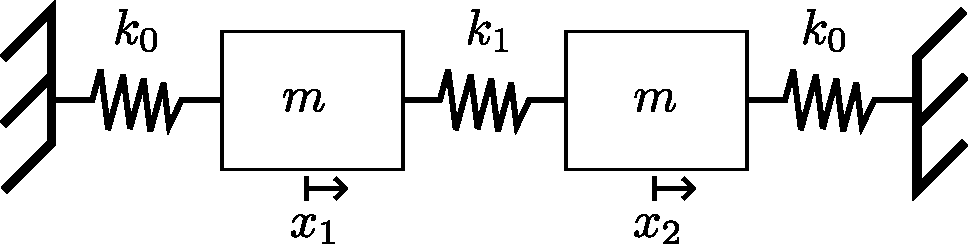
\includegraphics[width=0.4\paperwidth]{figures/coupled-oscillators-diagram}
\par\end{center}

By inspection, the equations of motion are:
\begin{eqnarray}
m\ddot{x}_{1} & = & -k_{0}x_{1}+k_{1}(x_{2}-x_{1})\\
m\ddot{x}_{2} & = & -k_{0}x_{2}-k_{1}(x_{2}-x_{1})
\end{eqnarray}
which may be written in matrix form as
\begin{equation}
\mathbf{\ddot{x}}=\frac{1}{m}\left[\begin{array}{cc}
-(k_{0}+k_{1}) & k_{1}\\
k_{1} & -(k_{0}+k_{1})
\end{array}\right]\mathbf{x}
\end{equation}
Because of the form of the matrix%
\footnote{The matrix $\left[\begin{array}{cc}
a & b\\
b & a
\end{array}\right]$ has eigenvectors $\left(\begin{array}{c}
1\\
1
\end{array}\right)$ and $\left(\begin{array}{c}
1\\
-1
\end{array}\right)$ with eigenvalues $(a+b)$ and $(a-b)$.%
}, we can immediately see that it has eigenvectors corresponding to
common and differential motion, with eigenvalues $\left\{ -k_{0},-(k_{0}+2k_{1})\right\} $. 

Applying this diagonalization, we find:
\[
\mathbf{\ddot{x'}}=\frac{1}{m}\left[\begin{array}{cc}
-k_{0} & 0\\
0 & -(k_{0}+2k_{1})
\end{array}\right]\mathbf{x'}\text{ where }\mathbf{x'}=\left[\begin{array}{cc}
1 & 1\\
1 & -1
\end{array}\right]\mathbf{x}
\]
The presence of the coupling $k_{1}$ only affects the differential
mode.


%% \subsection{Damped oscillators}

%% Now consider a mass connected to the wall via a spring with spring
%% constant $k$ and a velocity damper with damping constant $\gamma$:

%% \begin{center}
%% 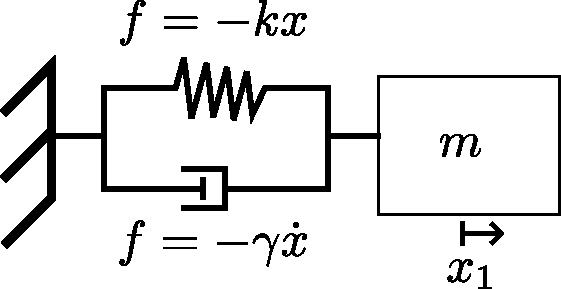
\includegraphics[width=0.25\paperwidth]{figures/damped-oscillator-diagram}
%% \par\end{center}

%% The equation of motion of the mass is:
%% \begin{equation}
%% m\ddot{x}=-kx-\gamma\dot{x}+f_{external}
%% \end{equation}
%% with Laplace transform
%% \begin{equation}
%% ms^{2}X=-kX-\gamma sX+F_{external}
%% \end{equation}
%% giving rise to a transfer function of

%% \begin{eqnarray*}
%% \frac{X}{F} & = & \frac{1}{ms^{2}+\gamma s+k}\\
%%  & = & \left(\frac{1}{m}\right)\frac{1}{\left(s-s_{+}\right)\left(s-s_{-}\right)}\text{ with }s_{\pm}=-\frac{1}{2}\frac{\gamma}{m}\pm\frac{1}{2}\sqrt{\left(\frac{\gamma}{m}\right)^{2}-4\frac{k}{m}}
%% \end{eqnarray*}


%% \subsection{Optical damping}

%% Suppose the cavity mirrors are traveling away from each other with
%% a velocity $v$. Then the phase of the reflected beam is changing
%% at a rate $\left(2\pi/\lambda\right)2v$. We can interpret this as
%% the light being Doppler shifted by $\Delta\omega=\left(2\pi/\lambda\right)2v$.
%% This optical frequency shift will cause the cavity to be closer or
%% further to resonance as compared to a cavity with stationary mirrors.

%% From this we can calculate the optical damping coefficient $\gamma$:

%% \[
%% \gamma\equiv-\frac{\partial f}{\partial v}=-\frac{\partial}{\partial v}\frac{2P}{c}=-\frac{2}{c}\frac{\partial\phi}{\partial v}\frac{\partial P}{\partial\phi}
%% \]
%% where $\frac{\partial\phi}{\partial v}=\frac{\partial\phi}{\partial\omega}\frac{\partial\omega}{\partial v}=\left(1/fsr\right)\left(4\pi/\lambda\right)$
%% so
%% \[
%% \gamma=\frac{2}{c}\frac{1}{fsr}\frac{4\pi}{\lambda}2Fg^{2}\frac{\cos(\phi)\sin(\phi)}{\left(1+F\sin^{2}\phi\right)^{2}}P_{IN}
%% \]

\begin{figure}
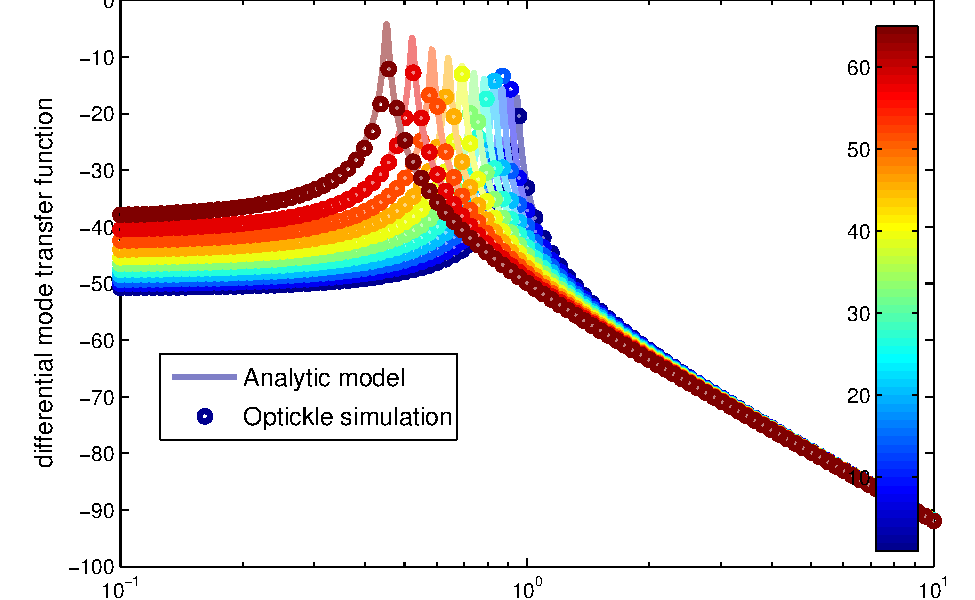
\includegraphics[width=\columnwidth]{figures/model-comparison}
\caption[Optical spring transfer function (numerical and analytic)]{\label{fig:model-comparison}The optical spring effect:  As a cavity is detuned from resonance, the resonance of the differential mode deceases.  This figure compares the resultsof a numerical  (Optickle) model with analytic results. The units of the
  y-axis are $20\log_{10}$(displacement/force); the x-axis is Hz;
  color indicates cavity detuning in picometers.}
\end{figure}


\section{Gaussian beams}

The general picture of Gaussian beams is shown here:

It is convenient to introduce the complex beam parameter $q$.  In terms of $q$:
\begin{equation}
\frac{1}{q(z)} = \frac{1}{R(z)} - i \frac{\lambda}{\pi w^2(z)}
\end{equation}
where $R(z)$ is the radius of curvature of the phase fronts at a
position $z$ along the optical axis, and $w(z)$ is the spot size at
that location.  We can also write:
$q(z) = i z_R + (z - z_0)$.

For a mode to resonate in an optical cavity, the spherical surface of
the mirrors must match the spherical phase front of the beam at the
location of the mirror.

Suppose mirror 1 has curvature $R_1$ and coordinate $z_1$, and
similarly for mirror 2.  We would like to solve for the waist location
and Rayleigh range.

References: Kogelnik and Li \cite{Kogelnik1966Laser}, Siegman \cite{Siegman1990Lasers}, \cite{Rudiger1998Phase,Fox1961Resonant}.

\section{Laser modes}

The eigenmodes of an optical cavity formed from spherical lenses are
the Hermite-Gauss (if the cavity has rectangular symmetry) or
Laguerre-Gauss (for axial symmetry) modes.  The amplitude distribution
at the beam waist is a Gaussian multiplied by a Hermite or Laguerre
polynomial.  These are exactly the same familes of functions as the
energy eigenstate wavefunctions of the simple harmonic oscillator in
quantum mechanics.

\begin{comment}
\section{Feedback control}

Operation of the LIGO detectors relies crucially on feedback control
systems.  In general, the response of the optical plant is completely
nonlinear; in order to produce a valid readout, the plant must be held
very close to its operating point.  The use of feedback control allows
us to attain linear response from an otherwise very nonlinear machine.

Here is a basic diagram of a feedback system:

Algebraically, one can derive a relationship giving the transfer function
of the closed-loop system in the Laplace domain:
\end{comment}

\section{The Antenna Pattern and the FSR}
\label{sec:antenna-pattern}
Gravitational waves come in two polarizations; for waves impinging
from a given direction, the second polarization represents an ellipse
of oscillating transverse strains rotated 45 degrees relative to the
first.  

Fundamentally, a Michelson interferometer is sensitive to two
polarizations of gravitational waves.  However, as discussed in chapter~\ref{chapter2}, we
elect to throw away sensitivity to one polarization in return for
common-mode noise immunity in the second polarization.

Although the waves come in two polarizations, one should note that
there is no globally consistent notion of \emph{the} $h_+$ and
$h_\times$ polarizations.  This is forbidden by the Hairy Ball
theorem.  

For a single detector, we can identify $h_+$ as the polarization
that shows up in DARM, and $h_\times$ as the polarization that would
show up in CARM.  Immediately (again due to the hairy ball theorem) we
see that there must be nulls in the sensitivity pattern of a single
interferometer.

In section~\ref{sec:long-wavelength}, we introduced the \emph{long
  wavelength approximation}, in which we assume that the gravitational
wave phase changes slowly compared to the time required for light to
travel from one end of an interferometer arm to the other end.  This
approximation holds in the LIGO detection band ($f \lesssim 7000$ Hz
corresponds to $\lambda \gtrsim 40$ km) but fails completely for GW
frequencies equal to the free spectral range of the arm cavities,
where the GW wavelength exactly matches the arm length.  For a
normally incident GW at this frequency, a photon traversing the arm
will see an elongated optical path length on its trip down the arm but
a contracted path length on its return trip, yielding zero net effect.
The antenna pattern is therefore a frequency-dependent function; to
calculate it, we must consider the spatial extent and time evolution
of the gravitational wave.

%% FIXME: References to cite:
%% \cite{Giampanis2008Search,Schilling1997Angular,Rakhmanov2008Highfrequency,Butler2004Characterization,Fricke2007HighFrequency}

\section{Shot Noise}
The root-mean-square of a Poisson process with current $I$ and quantum
$q$ measured over a bandwidth of $\Delta f$ is 
$$\sigma = \sqrt{2 q I \Delta f}$$ 
Here $I$ could be the electric current in Amps (=Coulombs/second) and
$q$ the charge of an electron.  For light incident on a photodiode,
the photon shot noise can be considered as an energy current, with
$I\leftarrow P$ being the DC power, and $q\leftarrow h\nu$ being the
energy per photon.

The amplitude spectral density of this process is white, with
amplitude $\sqrt{2qI}$ in units of [I] per square root of Hz.
For power $P$, the shot noise amplitude spectral density is 
\begin{equation}
\text{shot noise ASD} = \sqrt{2 h\nu P}\quad [\text{Watts}/\sqrt{\text{Hz}]}
\label{eq:shotnoise-asd}
\end{equation}
which gives a relative intensity noise of $\sqrt{2 h\nu/P}$.

\begin{comment}
\section{Noise analysis of opamp circuits}

\begin{figure}
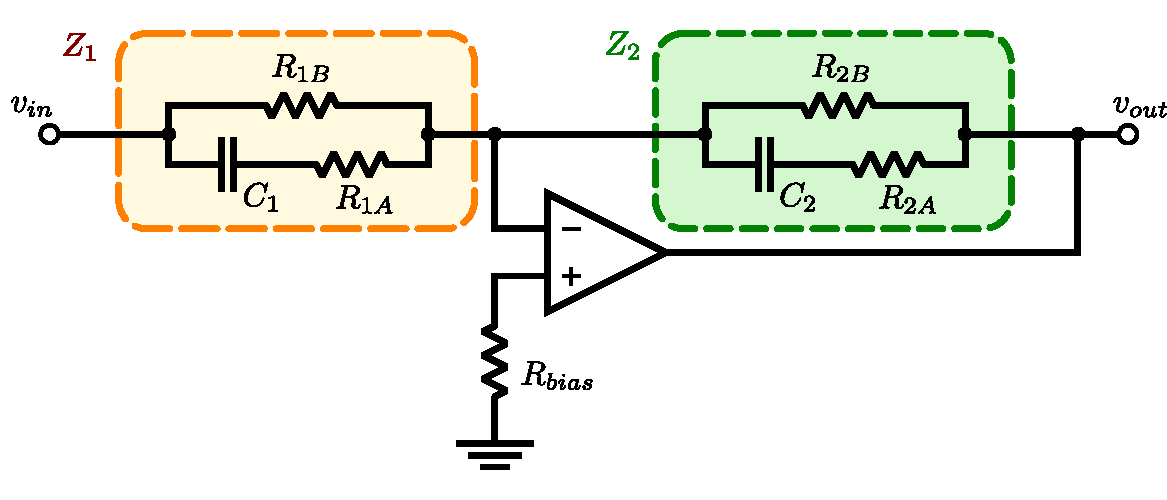
\includegraphics[width=\columnwidth]{notes/figures/inverting-amp.pdf}
\caption{\label{fig:inverting-amp}Basic active filter in the inverting amplifier configuration.} 
\end{figure}

Cite: Art of Electronics\cite{ArtOfElectronics}
\end{comment}
%\cite{Quetschke2007Complex}
%\cite{Williams1972Optics}
